%%%%%%%%%%%%%%%%%%%%%%%%%%%%%%%%%%%%%%%%%
% Journal Article
% LaTeX Template
% Version 1.4 (15/5/16)
%
% This template has been downloaded from:
% http://www.LaTeXTemplates.com
%
% Original author:
% Frits Wenneker (http://www.howtotex.com) with extensive modifications by
% Vel (vel@LaTeXTemplates.com)
%
% License:
% CC BY-NC-SA 3.0 (http://creativecommons.org/licenses/by-nc-sa/3.0/)
%
%%%%%%%%%%%%%%%%%%%%%%%%%%%%%%%%%%%%%%%%%

%----------------------------------------------------------------------------------------
%	PACKAGES AND OTHER DOCUMENT CONFIGURATIONS
%----------------------------------------------------------------------------------------

\documentclass[twoside, twocolumn]{article}

\usepackage{blindtext} % Package to generate dummy text throughout this template

\usepackage[sc]{mathpazo} % Use the Palatino font
\usepackage[T1]{fontenc} % Use 8-bit encoding that has 256 glyphs
\linespread{1.05} % Line spacing - Palatino needs more space between lines
\usepackage{microtype} % Slightly tweak font spacing for aesthetics

\usepackage[english]{babel} % Language hyphenation and typographical rules

\usepackage[hmarginratio=1:1,top=32mm,columnsep=20pt]{geometry} % Document margins
\usepackage[hang, small,labelfont=bf,up,textfont=it,up]{caption} % Custom captions under/above floats in tables or figures
\usepackage{booktabs} % Horizontal rules in tables

\usepackage{lettrine} % The lettrine is the first enlarged letter at the beginning of the text

\usepackage{amsmath}
\usepackage{graphicx}

\usepackage{enumitem} % Customized lists
\setlist[itemize]{noitemsep} % Make itemize lists more compact

\usepackage{abstract} % Allows abstract customization
\renewcommand{\abstractnamefont}{\normalfont\bfseries} % Set the "Abstract" text to bold
\renewcommand{\abstracttextfont}{\normalfont\small\itshape} % Set the abstract itself to small italic text

\usepackage{titlesec} % Allows customization of titles
\renewcommand\thesection{\Roman{section}} % Roman numerals for the sections
\renewcommand\thesubsection{\roman{subsection}} % roman numerals for subsections
\titleformat{\section}[block]{\large\scshape\centering}{\thesection.}{1em}{} % Change the look of the section titles
\titleformat{\subsection}[block]{\large}{\thesubsection.}{1em}{} % Change the look of the section titles

\usepackage{fancyhdr} % Headers and footers
\pagestyle{fancy} % All pages have headers and footers
\fancyhead{} % Blank out the default header
\fancyfoot{} % Blank out the default footer
\fancyhead[C]{Project 2 $\bullet$ Borries, Thiel, Schw\"ar $\bullet$ WS 2016/17} % Custom header text
\fancyfoot[RO,LE]{\thepage} % Custom footer text

\usepackage{titling} % Customizing the title section

\usepackage{hyperref} % For hyperlinks in the PDF

%----------------------------------------------------------------------------------------
%	TITLE SECTION
%----------------------------------------------------------------------------------------

\setlength{\droptitle}{-4\baselineskip} % Move the title up

\pretitle{\begin{center}\Huge\bfseries} % Article title formatting
\posttitle{\end{center}} % Article title closing formatting
\title{Machine Learning - Deep Learning Project 2} % Article title
\author{%
\textsc{Anton Borries} \\[1ex]
\normalsize 2204600 \\
\normalsize  \href{mailto:anton.borries@hhu.de}{anton.borries@hhu.de}
\and
\textsc{Johannes Thiel} \\[1ex]
\normalsize 2164216 \\
\normalsize \href{mailto:johannes.thiel@hhu.de}{johannes.thiel@hhu.de}
\and
\textsc{Simon Schw\"ar} \\[1ex]
\normalsize extern (HSD/RSH) \\
\normalsize \href{mailto:simon.schwaer@hs-duesseldorf.de}{simon.schwaer@hs-duesseldorf.de}
}

\date{\today} % Leave empty to omit a date
\renewcommand{\maketitlehookd}{%
\begin{abstract}
\noindent We train a neural Network to recognize images from the CIFAR-10 dataset. \\
Additionally, we take a look at Recurrent Neural Networks using Long Short-Term Memory cells and use them to predict an arbitrary dataset and the international airline passenger volume.
\end{abstract}
}

%----------------------------------------------------------------------------------------

\begin{document}

% Print the title
\maketitle

%----------------------------------------------------------------------------------------
%	ARTICLE CONTENTS
%----------------------------------------------------------------------------------------

\section{Architecture}

\lettrine[nindent=.2em,lines=2]{O} ur network consists of 5 total layers. The first two are both convolutional layers and the latter are fully connected. \\
We make use of 2 x 2 pooling and local response normalization between the two convolutional layers. \\
The whole network has about 1 million parameters. \\
We found that increasing the size of the fully connected layers did not result in greater accuracy, so we chose a small size for them to speed up the training process. \\
We used ReLu as our activation function for all layers.

\begin{table}[htb]
\label{table_conv}
	\caption{Convolutional Layers}
	\centering
		\begin{tabular}{l l l l}
			Layer & 1 & 2 \\
			\midrule
			Input Size & 32 x 32 & 16 x 16 \\
			Filter Size & 5 x 5 & 5 x 5 \\
			Output Channels & 64 & 64 \\
			Pooling & 2 x 2 & 2 x 2 \\
			Activation Function & ReLu & ReLu \\
\end{tabular}
\end{table}

\begin{table}[htb]
\label{table_fcl}
	\caption{Fully Connected Layers}
	\centering
		\begin{tabular}{l l l l}
			Layer & 3 & 4 & 5\\
			\midrule
			Input Size & 8 x 8 x 64 & 256 & 128 \\
			Activation Function & ReLu & ReLu & ReLu \\
			Dropout & No & No & No\\
\end{tabular}
\end{table}

%------------------------------------------------

\section{Training}

We used a batch size of 128 to train our network. \\
For the loss function we decided to use the cross entropy method.

\begin{equation}
 C = - \dfrac{1}{n} \sum_{z} [y \ln a + (1 - y) \ln (1 - a)]
\end{equation}

This is helping us to avoid the learning slowdown \cite{crossentro}.\\
We utilized the Adam optimizer with a learning rate of $0.001$ to train the network. \\
Using a higher learning rate resulted in pretty poor results of about 15\% test accuracy.

%------------------------------------------------

\section{Evaluation}
We evaluate our network by testing against the 10000 test images in the CIFAR-10 dataset. \\
With a low amount of opimization iterations we get varying results. For example with 500 batches of optimization we get a test accuracy between 30\% up to 36\% \\
Increasing the amount of iterations we found the reulst to be both better and more stable. \\
Going up to 2500 iterations we achive a test accuracy of 54\% - 56\% and with 20000 iteration we reached a test accuracy of 68.78\%.



%------------------------------------------------

\section{Other architectures}
We tried out another architecure. It is similar to our previous one but uses 3 x 3 convolutional filters and has an additional convolutional layer. We did not apply max pooling after this layer as it didn't improve our performance. \\


\begin{table}[htb]
\label{table_conv}
	\caption{Convolutional Layers}
	\centering
		\begin{tabular}{l l l l}
			Layer & 1 & 2 & 3\\
			\midrule
			Input Size & 32 x 32 & 16 x 16  & 8 x 8\\
			Filter Size & 3 x 3 & 3 x 3 & 3 x 3\\
			Output Channels & 64 & 64 & 64\\
			Pooling & 2 x 2 & 2 x 2 & None\\
			Activation Function & ReLu & ReLu \\
\end{tabular}
\end{table}

\begin{table}[htb]
\label{table_fcl}
	\caption{Fully Connected Layers}
	\centering
		\begin{tabular}{l l l l}
			Layer & 4 & 5 & 6\\
			\midrule
			Input Size & 8 x 8 x 64 & 256 & 128 \\
			Activation Function & ReLu & ReLu & ReLu \\
			Dropout & No & No & No\\
\end{tabular}
\end{table}

%------------------------------------------------

\section{Dataset Distortion}

We applied distortion to every batch at runtime to increase the size of our dataset. For this we changed the hue, flipped the image and changed the brightness. \\
We could not observe any significant increase in our accuracy by doing this.
We think this is the case because we did not run enough training iterations to make effective use of having more data.

%------------------------------------------------

\section{Dropout}

We tried applying a dropout layer for both our networks. This resulted in worse accuracy accross the board. \\
This might be because of our fully connected layers being rather small and maybe not having enough parameters after dropout to learn the data.

%------------------------------------------------

\section{Visualization}

We visualize our network using Tensorboard.

\begin{figure}[htb]
\centering
	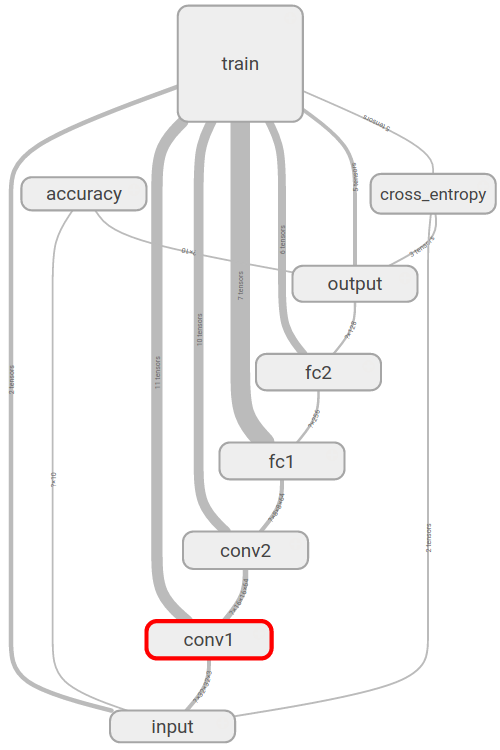
\includegraphics[width=0.48\textwidth]{network.png}
	\caption{Full network}
\end{figure}

\begin{figure}[htb]
\centering
	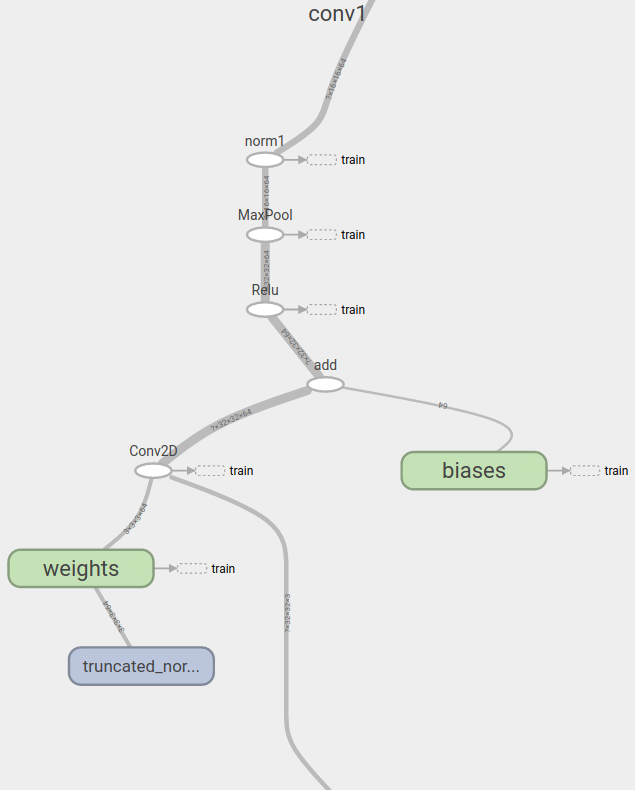
\includegraphics[width=0.48\textwidth]{conv_layer.png}
	\caption{The first convolutional layer}
\end{figure}

\begin{figure}[htb]
\centering
	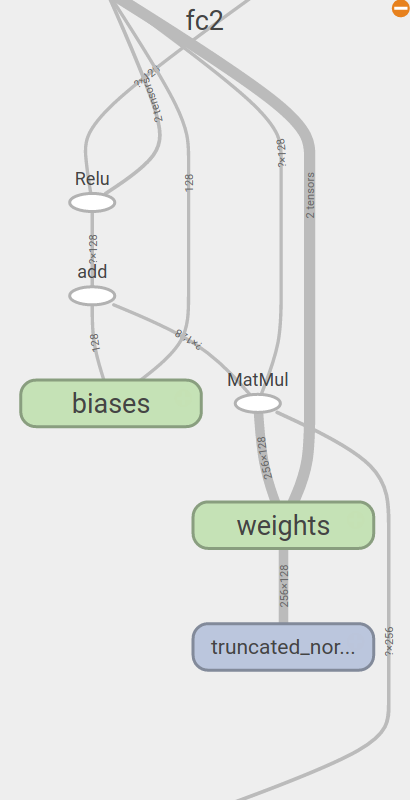
\includegraphics[width=0.48\textwidth]{fc_layer.png}
	\caption{The first fully connected layer}
\end{figure}




%------------------------------------------------

\section{Recurrent Neural Network Architecture}
We chose a very minimalist architecture for this task as it already provides good results and our tests showed that stacking more LSTM cells did not provide better results. \\
We use one LSTM cell followed by a fully connected layer with one unit.

\begin{figure}[htb]
\centering
	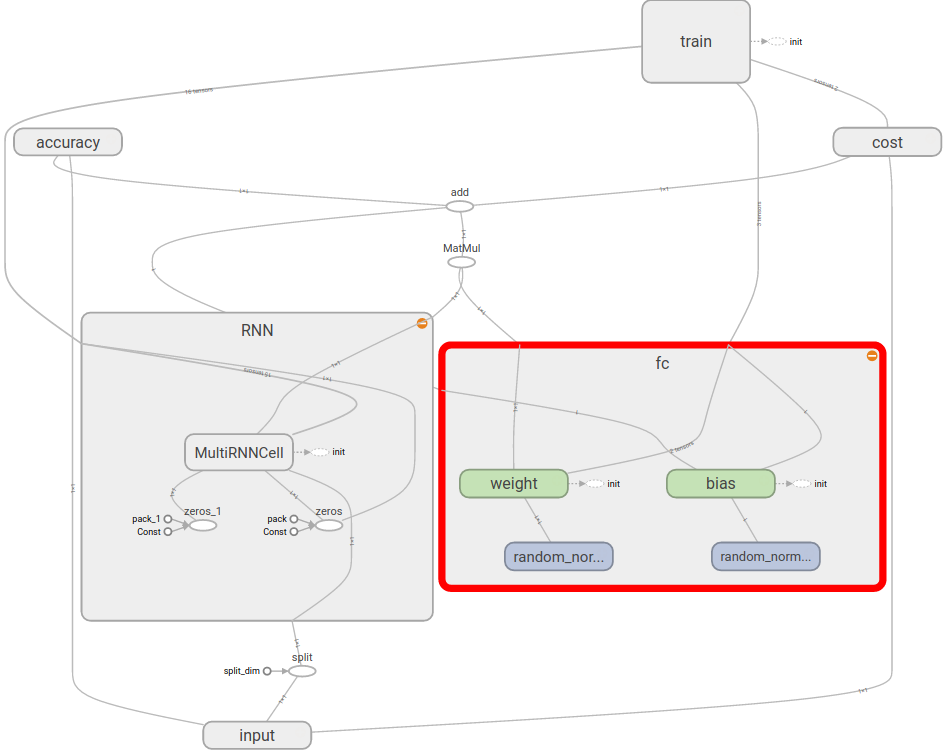
\includegraphics[width=0.48\textwidth]{rnn.png}
	\caption{Visualization of our RNN}
\end{figure}


%------------------------------------------------

\section{LSTM Cells}
The concept of Long Short Term Memory cells is to give the network a memory of previous inputs, so they can be used to make predictions. \\
The LSTM cells have a hidden state that can be used to "memorize" information. During training, the network learns which information to keep. \\
A LSTM takes three inputs:
\begin{itemize}
\item the normal input
\item the output of the previous cell
\item the hidden state of the previous cell
\end{itemize}

%------------------------------------------------

\section{Training}
We use the first 700 data entries for our training set and the last 300 datapoints for our test set. \\
As cost function we use the Mean Squared Error and optimize with the Adam optimizer. \\
After training our network on the first 700 datapoints, we evaluate it using our test set. Over the whole test set we get an average MSE of ~0.000159.

%------------------------------------------------

\section{Prediction Fit}
Plotting our prediction and the ground truth visualizes the performance of our network. \\
We can see that it is able to accurately predict the frequency of the curve but it seems to have a little offset on the y-axis

\begin{figure}[htb]
\centering
	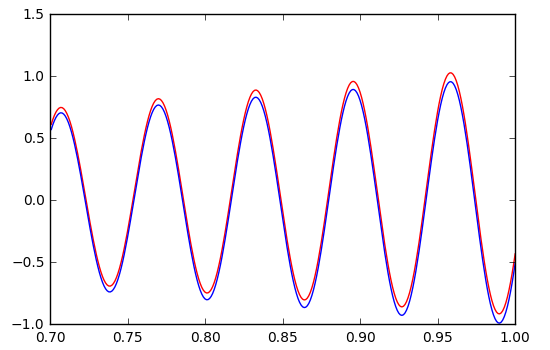
\includegraphics[width=0.48\textwidth]{rnn_fit.png}
	\caption{The red line is our prediction, the blue one is the ground truth}
\end{figure}


\section{Real World Example}

We chose a dataset of international airline passengers as a real world example for using Recurrent Neural Networks with LSTM cells. \\
The dataset contains the amount of international airline passengers for every month from 1949 until 1960. We can observe a general upwards trend with periodic spikes. \\
For this task we used a RNN architecture similar to the one previously used but stacked 5 LSTM cells as this provided a good improvement over just using one. \\
We split up the data in a trainig and a test set. The training set contains the first 100 datapoints and the test set contains the other 44 datapoints. \\
After training we evaluate the network with our test set and get and average MSE of ~0.141. Looking at the predicition fit the network is able to accuratly predict the general trend and frequency of the spikes.

\begin{figure}[htb]
\centering
	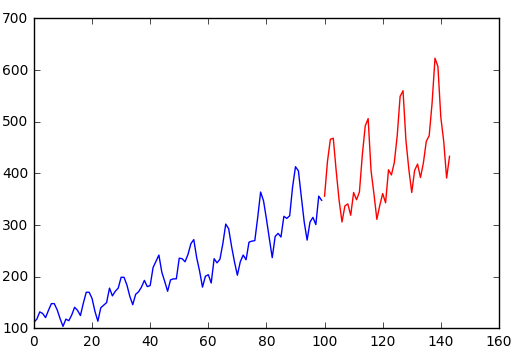
\includegraphics[width=0.48\textwidth]{rnn_plane_fit.png}
	\caption{The red line is our prediction, the blue one is the ground truth}
\end{figure}

%----------------------------------------------------------------------------------------
%	REFERENCE LIST
%----------------------------------------------------------------------------------------

\begin{thebibliography}{99} % Bibliography - this is intentionally simple in this template

\bibitem{crossentro}Cross Entropy,\\ \url{http://neuralnetworksanddeeplearning.com/chap3.html}, 06 12 2016.

\end{thebibliography}

%----------------------------------------------------------------------------------------
\end{document}


